\documentclass[border=0.2cm]{standalone}
\usepackage{tikz}
\usetikzlibrary{automata, positioning}

\title{fsm}

\begin{document}
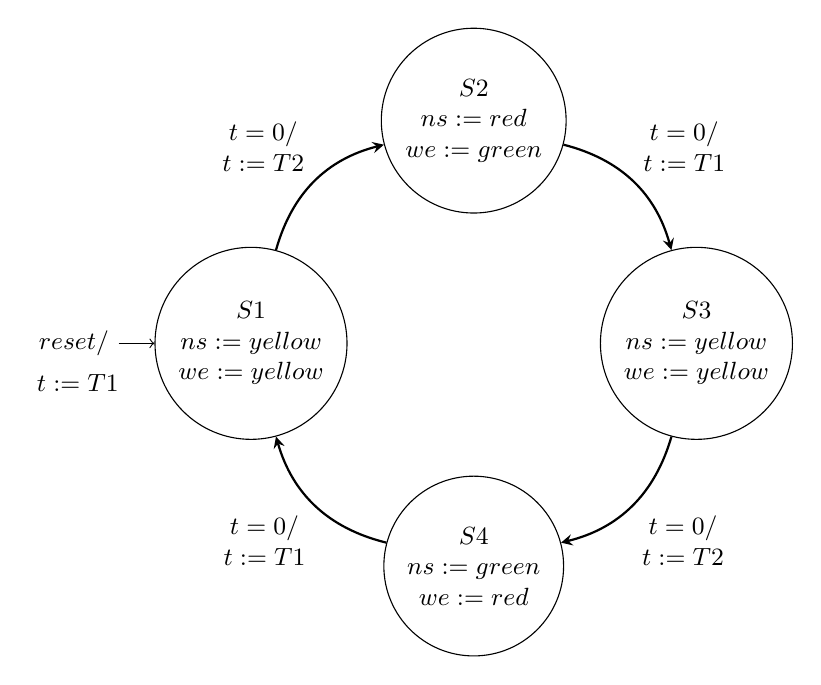
\begin{tikzpicture} [node distance = 4cm, on grid, auto, font=\small]
    \node (s1)
        [state, initial left, initial text = {$reset/$}, align=center]
        {$S1$ \\$ns:=yellow$ \\ $we:=yellow$};
    \node (s2)
        [state, above right = of s1, align=center]
        {$S2$ \\ $ns:=red$\\$we:=green$};
    \node (s3)
        [state, below right = of s2, align=center]
        {$S3$ \\ $ns:=yellow$\\$we:=yellow$};
    \node (s4)
        [state, below left = of s3, align=center]
        {$S4$ \\ $ns:=green$\\$we:=red$};

    \path [-stealth, thick]
    (s1) edge [bend left] node [align=center] {$t=0/$\\$t:=T2$} (s2)
    (s2) edge [bend left] node [align=center] {$t=0/$\\$t:=T1$} (s3)
    (s3) edge [bend left] node[align=center] {$t=0/$\\$t:=T2$} (s4)
    (s4) edge [bend left] node[align=center] {$t=0/$\\$t:=T1$} (s1)
    ;
    \node[align=left] at (-2.2,-0.5) {$t:=T1$};
\end{tikzpicture}
\end{document}